% !TEX root = ../thesis.tex

\chapter{Systémová príručka}

\section{Funkcia platforiem}

Platformy nasadené v rámci bakalárskej práce sú určené na nasadenie úloh strojového učenia zdrojových kódov Python. Pre správnu funkčnosť je nutné správne implementovať tieto platformy a pripojiť ďalšie stroje. Riadiaca rovina Kubernetes sa postará o viacero aspektov. Plánovanie týchto úloh a na ktorom pracovnom stroji sa daná úloha bude riešiť a za akých podmienok. Kubeflow ma schopnosť návrhu zdrojových kódov a konvertovanie týchto kódov pre pipelines, aby bolo možné ich nasadenie na systém Kubernetes.

\section{Inštalácia riadiacej roviny Kubernetes}

\subsection*{Systémové požiadavky}

Na inštaláciu platformy Kubernetes ako riadiací uzol je náležitosťou, aby stroj spĺňal minimálne systémové požiadavky:

\begin{itemize}
    \item Operačný systém: \textbf{Ubuntu 18.04 LTS a vyšší}
	\item Počet jadier procesora: \textbf{2}
    \item Veľkosť operačnej pamäte RAM: \textbf{12GB}
    \item Veľkosť pamäťového úložiska: \textbf{50GB}
\end{itemize}

\subsection*{Postup inštalácie}
\label{sec:hello}

Inštalácia je vykonávaná v terminály Ubuntu v nasledovnom poradí:
\begin{enumerate}
    \item{\noindent Odporúča sa prejsť do režimu \textbf{root} vykonaním príkazu a zadaním hesla.
\begin{lstlisting}[language=Bash,basicstyle=\footnotesize]
    sudo -s
    \end{lstlisting}}
\item{\noindent Nastavenie pravidiel firewallu, aby bol viditeľný premostený prenos.
\begin{lstlisting}[language=Bash,basicstyle=\footnotesize]
    cat <<EOF | sudo tee /etc/modules-load.d/k8s.conf
    br_netfilter
    EOF

    cat <<EOF | sudo tee /etc/sysctl.d/k8s.conf
    net.bridge.bridge-nf-call-ip6tables = 1
    net.bridge.bridge-nf-call-iptables = 1
    EOF
    sudo sysctl --system
    \end{lstlisting}}
    \item{\noindent Kvôli Kubeadm je potrebné zakázať swap na všetkých uzloch.
\begin{lstlisting}[language=Bash,basicstyle=\footnotesize]
    sudo swapoff -a
    sudo sed -i '/ swap / s/^\(.*\)$/#\1/g' /etc/fstab
    \end{lstlisting}}
    \item{\noindent Nasleduje inštalácia požadovaných balíkov pre Docker.
\begin{lstlisting}[language=Bash,basicstyle=\footnotesize]
    sudo apt-get update -y
    sudo apt-get install -y apt-transport-https ca-certificates \
        curl gnupg lsb-release
    \end{lstlisting}}
    \item{\noindent Pridanie kľúča Docker GPG a \acrshort{apt} repozitára.
\begin{lstlisting}[language=Bash,basicstyle=\footnotesize]
    curl -fsSL https://download.docker.com/linux/ubuntu/gpg | \
        sudo gpg --dearmor -o /usr/share/keyrings/\
        docker-archive-keyring.gpg

    echo \
        "deb [arch=amd64 signed-by=/usr/share/keyrings/\
        docker-archive-keyring.gpg] \
        https://download.docker.com/linux/ubuntu \
        $(lsb_release -cs) stable" | \
        sudo tee /etc/apt/sources.list.d/docker.list > /dev/null
\end{lstlisting}}
\item{\noindent Inštalácia samotnej komunitnej verzie Dockera.
\begin{lstlisting}[language=Bash,basicstyle=\footnotesize]
    sudo apt-get update -y
    sudo apt-get install docker-ce docker-ce-cli containerd.io -y
\end{lstlisting}}
\item{\noindent Pridanie konfigurácie Docker daemona pre použitie systemd ako cgroup ovládača.
\begin{lstlisting}[language=Bash,basicstyle=\footnotesize]
    cat <<EOF | sudo tee /etc/docker/daemon.json
    {
      "exec-opts": ["native.cgroupdriver=systemd"],
      "log-driver": "json-file",
      "log-opts": {
        "max-size": "100m"
      },
      "storage-driver": "overlay2"
    }
    EOF
\end{lstlisting}}
\item{\noindent Spustenie a povolenie služby ovládačov.
\begin{lstlisting}[language=Bash,basicstyle=\footnotesize]
    sudo systemctl enable docker
    sudo systemctl daemon-reload
    sudo systemctl restart docker
\end{lstlisting}}
\item{\noindent Dodanie potrebných nástrojov pre Kubeadm.
\begin{lstlisting}[language=Bash,basicstyle=\footnotesize]
    sudo apt-get update
    sudo apt-get install -y apt-transport-https /
        ca-certificates curl
    sudo curl -fsSLo \
        /usr/share/keyrings/kubernetes-archive-keyring.gpg \
        https://packages.cloud.google.com/apt/doc/apt-key.gpg
\end{lstlisting}}
\item{\noindent Pridanie kľúča GPG a repozitára \acrshort{apt} pre Kubeadm.
\begin{lstlisting}[language=Bash,basicstyle=\footnotesize]
    echo "deb \
        [signed-by=/usr/share/keyrings/\
        kubernetes-archive-keyring.gpg] \
        https://apt.kubernetes.io/ kubernetes-xenial main" | \
        sudo tee /etc/apt/sources.list.d/kubernetes.list
\end{lstlisting}}
\item{\noindent Inštalácia Kubelet, Kubeadm a kubectl služieb s verziou 1.21.12-00.
\begin{lstlisting}[language=Bash,basicstyle=\footnotesize]
    sudo apt-get update -y
    sudo apt-get install -y kubelet=1.21.12-00 \
    kubectl=1.21.12-00 kubeadm=1.21.12-00
\end{lstlisting}}
\item{\noindent Zablokovanie aktualizácie služieb pred nežiadanou aktualizáciou.
\begin{lstlisting}[language=Bash,basicstyle=\footnotesize]
    sudo apt-mark hold kubelet kubeadm kubectl
\end{lstlisting}}
\item{\noindent Inicializácia klastra využitím nástroja Kubeadm. Namiesto x.x.x.x je\br potrebné zadať IP adresu počítača. Vygeneruje sa token, ktorý je vhodné uchovať pre pripájanie ďalších strojov.
\begin{lstlisting}[language=Bash,basicstyle=\footnotesize]
    IPADDR="x.x.x.x"
    NODENAME=$(hostname -s)
    sudo kubeadm init --apiserver-advertise-address=$IPADDR \
        --apiserver-cert-extra-sans=$IPADDR  \
        --pod-network-cidr=192.168.0.0/16 \
        --node-name $NODENAME --ignore-preflight-errors Swap
\end{lstlisting}}
\item{\noindent Vytvorenie súboru kubeconfig pre službu kubectl na interakciu s klastrom.
\begin{lstlisting}[language=Bash,basicstyle=\footnotesize]
    mkdir -p $HOME/.kube
    sudo cp -i /etc/kubernetes/admin.conf $HOME/.kube/config
    sudo chown $(id -u):$(id -g) $HOME/.kube/config
\end{lstlisting}}
\item{\noindent Overenie funkcionality zobrazením spustených podov.
\begin{lstlisting}[language=Bash,basicstyle=\footnotesize]
    kubectl get po -n kube-system
\end{lstlisting}}
\item{\noindent Ako predvolené nastavenie sa aplikácie naplánujú na riadiacej rovine. Ak je žiadané nasadenie aj na riadiacej rovine nevyhnutné je vykonanie nasledujúceho príkazu.
\begin{lstlisting}[language=Bash,basicstyle=\footnotesize]
    kubectl taint nodes --all node-role.kubernetes.io/master-
\end{lstlisting}}
\item{\noindent Kubeadm neposkytuje žiaden sieťový prvok. Nakonfiguruje sa sieťový doplnok Calico.
\begin{lstlisting}[language=Bash,basicstyle=\footnotesize]
    kubectl apply -f \
        https://docs.projectcalico.org/manifests/calico.yaml
\end{lstlisting}}
\item{\noindent Kubernetes dashboard nie je predvolene nasadený. Pre nasadenie sa použije nasledovný príkaz.
\begin{lstlisting}[language=Bash,basicstyle=\footnotesize]
    kubectl apply -f \
        https://raw.githubusercontent.com/kubernetes/\
        dashboard/v2.5.0/aio/deploy/recommended.yaml
\end{lstlisting}}
\item{\noindent Pri používaní dashboardu sa vyžaduje vytvorenie používateľa, ktoré pozostáva z vytvorenia súborov a nasadenia do klastra.\br
\indent \textbf{admin-user.yaml:}
\begin{lstlisting}[language=Bash,basicstyle=\footnotesize]
    apiVersion: v1
    kind: ServiceAccount
    metadata:
        name: admin-user
        namespace: kubernetes-dashboard
\end{lstlisting}
\indent \textbf{clusterRoleBinding.yaml:}
\begin{lstlisting}[language=Bash,basicstyle=\footnotesize]
    apiVersion: rbac.authorization.k8s.io/v1
    kind: ClusterRoleBinding
    metadata:
        name: admin-user
    roleRef:
        apiGroup: rbac.authorization.k8s.io
        kind: ClusterRole
        name: cluster-admin
    subjects:
        - kind: ServiceAccount
        name: admin-user
        namespace: kubernetes-dashboard
\end{lstlisting}
\indent \textbf{Aplikovanie súborov:}
\begin{lstlisting}[language=Bash,basicstyle=\footnotesize]
    kubectl apply -f admin-user.yaml
    kubectl apply -f clusterRoleBinding.yaml
\end{lstlisting}}
\item{\noindent Vygenerovanie tokenu pre prihlásenie do dashboardu Kubernetes.
\begin{lstlisting}[language=Bash,basicstyle=\footnotesize]
    kubectl -n kubernetes-dashboard get secret $(kubectl -n \
        kubernetes-dashboard get sa/admin-user -o \
        jsonpath="{.secrets[0].name}") -o \
        go-template="{{.data.token | base64decode}}"
\end{lstlisting}}
\item{\noindent Po spustení tohto príkazu je prihlásenie možné zadaním tokenu prostredníctvom prehliadača na adrese\footnote{\url{http://localhost:8001/api/v1/namespaces/kubernetes-dashboard/services/https:kubernetes-dashboard:/proxy/}}.
\begin{lstlisting}[language=Bash,basicstyle=\footnotesize]
    kubectl proxy
\end{lstlisting}}
\item{\noindent Vytvorenie lokálneho trvalého zväzku a nastavenie predvoleného úložiska.
\begin{lstlisting}[language=Bash,basicstyle=\footnotesize]
    kubectl apply -f \
        https://raw.githubusercontent.com/rancher/local-path-\
        provisioner/master/deploy/local-path-storage.yaml
    kubectl patch storageclass local-path -p'\
        {"metadata":{"annotations":{"storageclass.\
        kubernetes.io/is-default-class":"true"}}}'
\end{lstlisting}}
\item{\noindent Overenie predošlého kroku je možné nasledovnými príkazmi.
\begin{lstlisting}[basicstyle=\footnotesize]
    kubectl -n local-path-storage get pod -o wide
    kubectl get sc
\end{lstlisting}}
\end{enumerate}

\section{Pripojenie pracovných strojov}

\subsection*{Systémové požiadavky}

\begin{itemize}
    \item Operačný systém: \textbf{Ubuntu 18.04 LTS a vyšší alebo Windows server 2019 a vyšší}
	\item Počet jadier procesora: \textbf{2}
    \item Veľkosť operačnej pamäte RAM: \textbf{2GB}
\end{itemize}

\subsection*{Linux/Ubuntu}

Pripojenie pracovného stroja Ubuntu je vykonávané v terminály Ubuntu v nasledovnom poradí:

\begin{enumerate}
\item{\noindent Vykonanie krokov \textbf{1. - 12.} z kapitoly \hyperref[sec:hello]{\textbf{Inštalácia riadiacej roviny Kubernetes}}}
\item{\noindent Vygenerovanie tokenu slúžiaceho na pripojenie stroja do klastra. Získanie tokenu použitím nasledovného príkazu na riadiacej rovine.
\begin{lstlisting}[basicstyle=\footnotesize]
    kubeadm token create --print-join-command
    \end{lstlisting}}
\item{\noindent Vytvorený token z riadiacej roviny sa spustí na stroji, ktorý je potrebné pripojiť. Znázornená je ukážka príkazu.
\begin{lstlisting}[basicstyle=\footnotesize]
    sudo kubeadm join 10.128.0.37:6443 \
        --token j4eice.33vgvgyf5cxw4u8i \
        --discovery-token-ca-cert-hash sha256:37f94469b58bcc\
        8f26a4aa44441fb17196a585b37288f85e22475b00c36f1c61
    \end{lstlisting}}
    \item{\noindent Kontrola úspešného pripojenia sa uskutoční spustením príkazu na riadiacej rovine pre výpis pripojených strojov.
\begin{lstlisting}[language=Bash,basicstyle=\footnotesize]
    kubectl get nodes
    \end{lstlisting}}
\end{enumerate}

\subsection*{Windows server}

Pri pripájaní stroja s operačným systémom Windows je nutné vykonať niektoré kroky na riadiacej rovine:

\begin{enumerate}
\item{\noindent Stiahnutie kontajnerovej sieti Flannel.
\begin{lstlisting}[basicstyle=\footnotesize]
    wget https://raw.githubusercontent.com/coreos/flannel/\
        master/Documentation/kube-flannel.yml
    \end{lstlisting}}
\item{\noindent Editácia net-conf.json sekcie, pridaním VNI a Portu v kube-flannel.yml.
\begin{lstlisting}[basicstyle=\footnotesize]
    net-conf.json: |
        {
            "Network": "10.244.0.0/16",
            "Backend": {
                "Type": "vxlan",
                "VNI": 4096,
                "Port": 4789
            }
        }
    \end{lstlisting}}
\item{\noindent Aplikovanie Flannel editovanej konfigurácie.
\begin{lstlisting}[language=Bash,basicstyle=\footnotesize]
    kubectl apply -f kube-flannel.yml
    \end{lstlisting}}
\item{\noindent Pridanie Flannelu a kube-proxy kompatibilné so systémom Windows s verziou 1.21.12, ktorá sa používa v tejto príručke.
\begin{lstlisting}[language=Bash,basicstyle=\footnotesize]
    curl -L https://github.com/kubernetes-sigs/sig-windows-tools\
        /releases/latest/download/kube-proxy.yml | \
        sed 's/VERSION/v1.21.12/g' | kubectl apply -f -
    kubectl apply -f https://github.com/kubernetes-sigs/sig-win\
        dows-tools/releases/latest/download/flannel-overlay.yml
    \end{lstlisting}}
\end{enumerate}

\noindent Ďalšie kroky sú vykonané v príkazovom riadku PowerShell ako administrátor:

\begin{enumerate}
\item{\noindent Inštalácia funkcie Containers. Po vykonaní tohto kroku sa vyžaduje reštartovanie.
\begin{lstlisting}[basicstyle=\footnotesize]
    Install-WindowsFeature -Name containers
    \end{lstlisting}}
\item{\noindent Nasledovná je inštalácia Dockera pre Windows serveri. Nutný je reštart.
\begin{lstlisting}[basicstyle=\footnotesize]
    Install-Module -Name DockerMsftProvider -Repository \
    PSGallery -Force
    Install-Package -Name docker -ProviderName DockerMsftProvider
    \end{lstlisting}}
\item{\noindent Stiahnutie a nasadenie služieb Wins, Kubelet a Kubeadm s verziou 1.21.12.
\begin{lstlisting}[language=Bash,basicstyle=\footnotesize]
    curl.exe -LO https://raw.githubusercontent.com/kubernetes-si\
        gs/sig-windows-tools/master/kubeadm/scripts/\
        PrepareNode.ps1
    .\PrepareNode.ps1 -KubernetesVersion v1.21.12
    \end{lstlisting}}
\item{\noindent Získanie tokenu použitím nasledovného príkazu na riadiacej rovine.
\begin{lstlisting}[language=Bash,basicstyle=\footnotesize]
    kubeadm token create --print-join-command
    \end{lstlisting}}
\item{\noindent Vytvorený token z riadiacej roviny sa spustí na stroji, ktorý je potrebné pripojiť. Znázornená je ukážka príkazu.
\begin{lstlisting}[basicstyle=\footnotesize]
    sudo kubeadm join 10.128.0.37:6443 \
        --token j4eice.33vgvgyf5cxw4u8i \
        --discovery-token-ca-cert-hash sha256:37f94469b58bcc\
        8f26a4aa44441fb17196a585b37288f85e22475b00c36f1c61
    \end{lstlisting}}
\item{\noindent Kontrola úspešného pripojenia sa uskutoční spustením príkazu na riadiacej rovine pre výpis pripojených strojov.
\begin{lstlisting}[language=Bash,basicstyle=\footnotesize]
    kubectl get nodes
    \end{lstlisting}}
\end{enumerate}

\section{Nasadenie Kubeflow do klastra Kubernetes}

Vykonané sú príkazy prostredníctvom riadiacej roviny v nasledovnom poradí:

\begin{enumerate}
\item{\noindent Pre nasadenie Kubeflow je potrebná služba Kustomize, vyžaduje sa stiahnutie súboru \textbf{kustomize-3.2.0-linux-amd64} z internetovej adresy\footnote{\url{https://github.com/kubernetes-sigs/kustomize/releases/tag/v3.2.0}}. Po stiahnutí sa súbor musí premenovať na \textbf{kustomize}}.
\item{\noindent Zmena práv súboru kustomize a presunutie do priečinka obsahujúce linuxové príkazy.
\begin{lstlisting}[basicstyle=\footnotesize]
    sudo chmod 755 kustomize
    sudo mv kustomize /bin
    \end{lstlisting}}
\item{\noindent Stiahnutie Git repozitára a prechod do priečinku.
\begin{lstlisting}[language=Bash,basicstyle=\footnotesize]
    git clone https://github.com/kubeflow/manifests.git
    cd manifests
    \end{lstlisting}}
\item{\noindent Nasadenie všetkých komponentov prostredníctvom príkazu.
\begin{lstlisting}[language=Bash,basicstyle=\footnotesize]
    while ! kustomize build example | kubectl apply -f -; \
        do echo "Retrying to apply resources"; sleep 10; done
    \end{lstlisting}}
\item{\noindent Po niekoľkých minútach, ak sú všetky pody spustené, je možné sa pripojiť prostredníctvom prehliadača na adrese\footnote{\url{http://localhost:8080}}. Predvolená prihlasovacia emailová adresa je \textbf{user@example} a heslo \textbf{12341234}.}
\end{enumerate}

\chapter{Používateľská príručka}

\section{Funkcia platforiem}
\subsection*{Požiadavky}

Na použitie tejto príručky sú nutné požiadavky ako:

\begin{itemize}
    \item Spustený Kubernetes a implementovaný Kubeflow
    \item Pripojenie na internet
    \item Webový prehliadač
\end{itemize}

\subsection*{Inštalácia}

Spočíva vo vykonaní postupnosti krokov, ktoré sa nachádzajú v systémovej príručke.

\section{Použitie platforiem}

\subsection*{Vytvorenie a spustenie vývojového prostredia}

Vykonanie tohto kroku je sprostredkované vďaka komponentu Notebooks. Používateľ klikne na rozhraní Kubeflow sekciu \textbf{Notebooks}. Zobrazia sa vytvorené prostredia, kde je znázornený ich status, aký obraz je nasadení, hardvérové využitie a tlačidla pre vypnutie, vymazanie alebo pripojenie k danému vývojovému prostrediu. Možno ich vidieť na obrázku \ref{notebook}.

Vytvorenie nového prostredia je uskutočnené stlačením tlačidla \textbf{New Notebook}, kde používateľ vyplní polia na základe svojich potrieb. Na výber je napríklad obraz, ktorý sa má spustiť na prostredí, veľkosť operačnej pamäte a úložiska. Nové prostredie sa vytvorí po kliknutí na tlačidlo \textbf{Launch}. Ak nové prostredie zmení svoj stav na \textbf{Running}, je možné sa pripojiť do daného prostredia a začať nasadzovať Python zdrojové kódy.

\begin{figure}[!h]
    \centering
    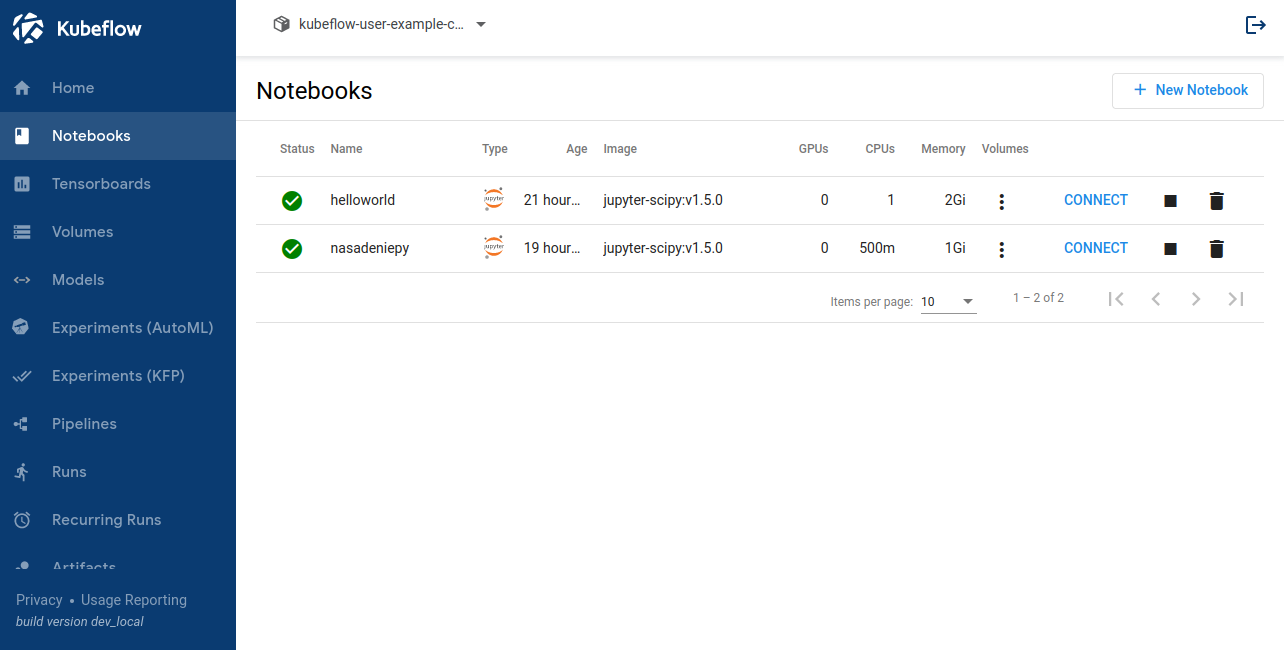
\includegraphics[width=1\linewidth]{figures/1.png}
    \caption{Pracovné prostredia - Notebooks}
    \label{notebook}
\end{figure}

\subsection*{Zostavenie pipelines z Python zdrojových kódov}

Pipelines sa zostavujú v pracovnom prostredí podobnému ako JupyterLab. Tento proces je nevyhnutný pre ďalší krok, kde sa nahráva pipeline do platformy Kubeflow. Na zostavenie je treba preformátovať Python funkcie na komponenty, aby boli pre Kubeflow zrozumiteľné. Formátovanie prebieha deklarovaním typu každého parametra pre funkcie, namiesto vrátenia objektu využívame objekt OutputhPath() a vytvorenie pipeline, kde popisuje postupnosť komponentov, ktoré sa majú volať, a parametre na ich odovzdanie. Nakoniec sa vykonáva konvertovanie Python pipeline do súboru YAML prostredníctvom nasledovného príkazu na JupyterLab pracovnom prostredí.

\begin{lstlisting}[basicstyle=\footnotesize]

    dsl-compile --py test_pipeline.py --output test_pipeline.yaml
    \end{lstlisting}

\subsection*{Implementovanie pipeline do Kubeflow}

Používateľ vyberie možnosť \textbf{Pipelines}. Na tejto obrazovke sa nachádzajú všetky nahraté pipelines s ich názvom a krátkym opisom. Vyberie možnosť \textbf{Upload pipeline}, kde vyplní názov, opis a nahrá samotnú pipeline v YAML formáte. Po nahratí sa začlení medzi ostatné a je možné ju spustiť na platforme. Kliknutím na jednu z pipelines sa zobrazí grafické znázornenie komponentov a postup krokov, ktoré sú znázornené na obrázku \ref{pipa}.

\begin{figure}[!h]
    \centering
    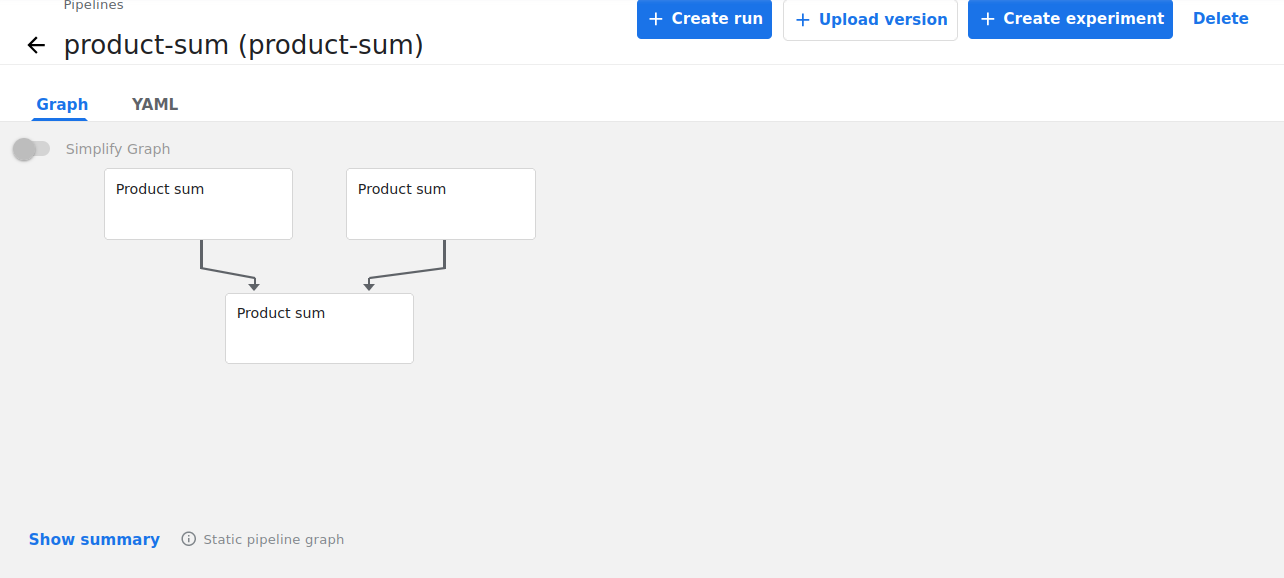
\includegraphics[width=1\linewidth]{figures/7.png}
    \caption{Grafické znázornenie súčtu a súčinu čísel}
    \label{pipa}
\end{figure}

\subsection*{Vytvorenie experimentu a chodu programu}

Pre vytvorenie experimentu sa musí používateľ presunúť do sekcie \textbf{Experiments (KFP)}. Následne klikne na tlačidlo \textbf{Create experiment}, kde zadá názov experimentu a pripadne aj opis. V ďalšom kroku je vytvorenie chodu programu vybranej pipeline. Na výber je chod programov, ktoré sa opakujú zadaným počtom opakovaní, alebo v určitom čase, alebo jednotný chod, ktorý sa spusti len raz. Po vytvorení experimentu je vidieť jednotlivé chody programov týchto pipelines vo vytvorenom experimente pre rozdelenie do logických skupín. Znázornené sú chody týchto programov, ich status a čas trvania na nasledujúcom obrázku \ref{exp}.

\begin{figure}[!h]
    \centering
    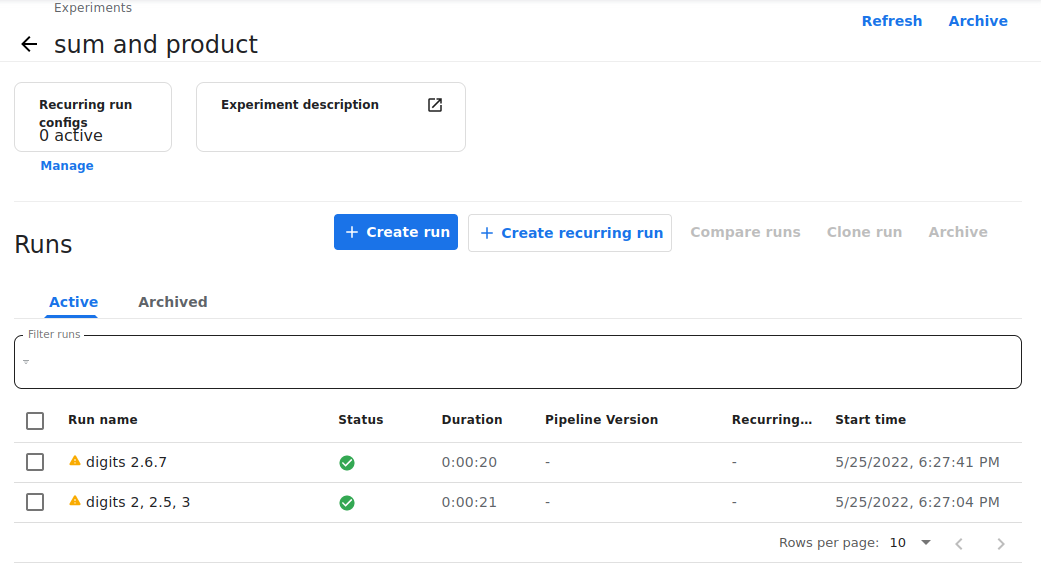
\includegraphics[width=1\linewidth]{figures/10.png}
    \caption{Experiment a chod programov súčtu a súčinu čísel}
    \label{exp}
\end{figure}

\subsection*{Zobrazenie chodu programu a výstupných údajov}

Po kliknutí na daný chod programu sa zobrazí postupnosť krokov. Každý krok môže obsahovať nejaký vstup a výstup. Možnosťou je daný beh programu archivovať, zrušiť alebo naklonovať s upravenými vstupnými parametrami pre rýchle nasadenie. Tieto možnosti sú na obrázku \ref{run}. Všetky výstupy sa nachádzajú v časti s názvom \textbf{Artifacts}.

\begin{figure}[!h]
    \centering
    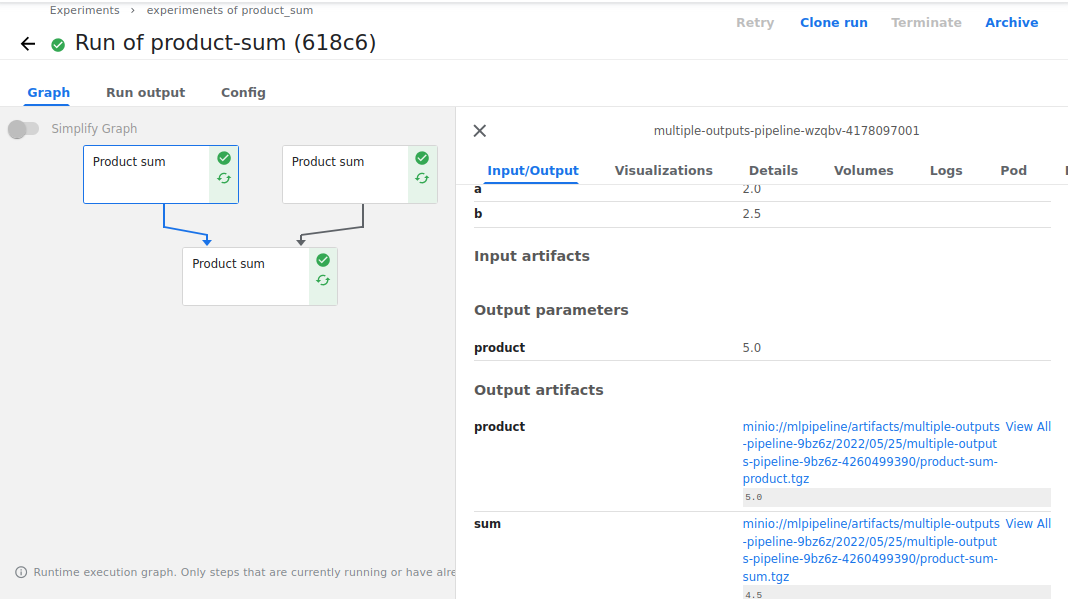
\includegraphics[width=1\linewidth]{figures/11.png}
    \caption{Vstupy a výstupy komponentov}
    \label{run}
\end{figure}

\section{Príklad použitia}

V tejto kapitole sa nachádza séria pokynov na nasadenie ukážkového Python zdrojového kódu na výpočet súčtu a súčinu čísel v nasledujúcom postupe krokov:

\begin{enumerate}
\item Vytvorenie pracovného prostredia kliknutím na sekciu \textbf{Notebooks} a následne \textbf{New Notebook}.
\item Zadanie názvu a výberu JupyterLab obrazu. Ostatné preferencie sú na potrebách používateľa. A kliknutie na \textbf{LAUNCH} nižšie.
\item Pripojenie k vytvorenému prostrediu kliknutím na tlačidlo \textbf{CONNECT}.
\item Nahranie súboru \textbf{product-sum.ipynb} priloženého na CD stlačením tlačidla \textbf{A} a spustenie celého nahratého Jupyter Notebook súboru spustením tlačidla \textbf{B} naznaceným na obrázku \ref{tu}.
\item {Stiahnutie vygenerovaného súboru kliknutím pravým tlačidlom myši na \textbf{product-sum.yaml} a výberom možnosti \textbf{Download}, tak ako je to znázornené na obrázku \ref{tu}.
\begin{figure}[!h]
    \centering
    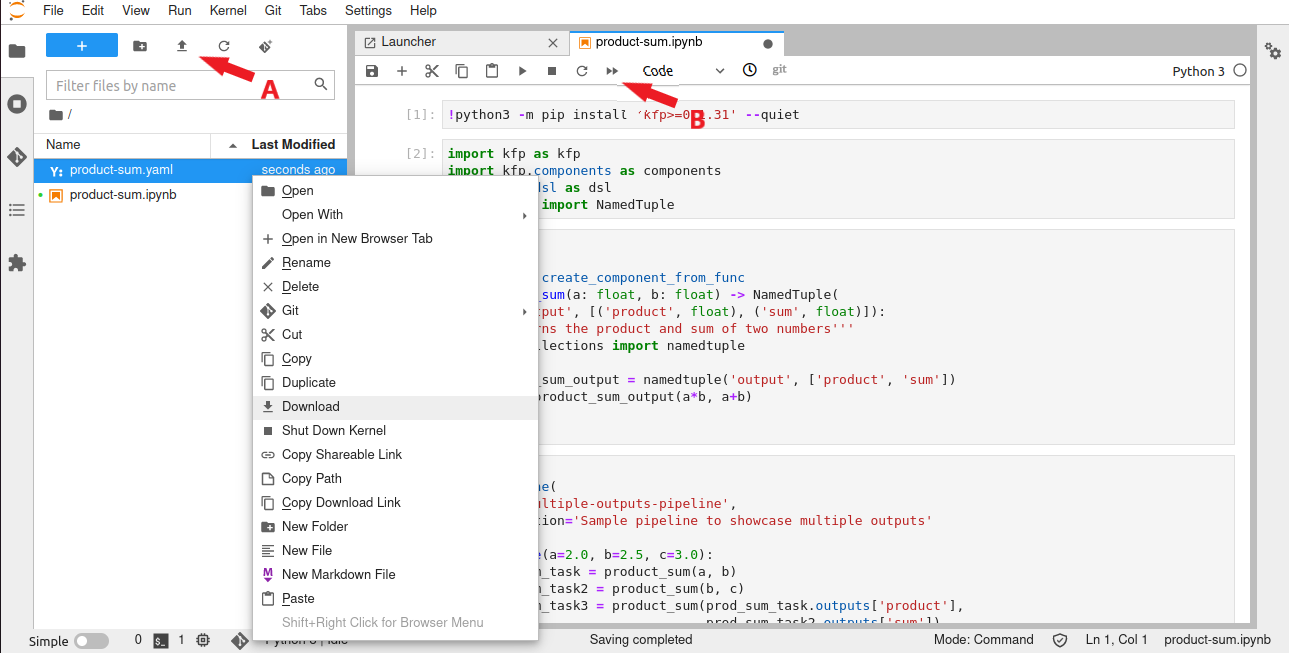
\includegraphics[width=1\linewidth]{figures/4.png}
    \caption{Prostredie JupyterLab}
    \label{tu}
\end{figure}}
\item Prechod do sekcie \textbf{Pipelines} a kliknutie tlačidla \textbf{Upload pipeline}.
\item Vypísanie názvu, nahranie stiahnutého súboru \textbf{product-sum.yaml} a stlačenie tlačidla \textbf{CREATE}.
\item Vytvorenie experimentu kliknutím na \textbf{Create experiment}.
\item Zadanie názvu Experimentu, stlačením \textbf{Next}.
\item Presunutím nižšie, zadaním ľubovoľných parametrov na sučet a súčin čísel a spustením \textbf{Start}.
\item Otvorenie vytvoreného chodu programu a vybratie ľubovoľného komponentu kliknutím, kde sa zobrazí vstup a výstup.
\end{enumerate}